% Options for packages loaded elsewhere
\PassOptionsToPackage{unicode}{hyperref}
\PassOptionsToPackage{hyphens}{url}
%
\documentclass[
]{article}
\usepackage{amsmath,amssymb}
\usepackage{iftex}
\ifPDFTeX
  \usepackage[T1]{fontenc}
  \usepackage[utf8]{inputenc}
  \usepackage{textcomp} % provide euro and other symbols
\else % if luatex or xetex
  \usepackage{unicode-math} % this also loads fontspec
  \defaultfontfeatures{Scale=MatchLowercase}
  \defaultfontfeatures[\rmfamily]{Ligatures=TeX,Scale=1}
\fi
\usepackage{lmodern}
\ifPDFTeX\else
  % xetex/luatex font selection
\fi
% Use upquote if available, for straight quotes in verbatim environments
\IfFileExists{upquote.sty}{\usepackage{upquote}}{}
\IfFileExists{microtype.sty}{% use microtype if available
  \usepackage[]{microtype}
  \UseMicrotypeSet[protrusion]{basicmath} % disable protrusion for tt fonts
}{}
\makeatletter
\@ifundefined{KOMAClassName}{% if non-KOMA class
  \IfFileExists{parskip.sty}{%
    \usepackage{parskip}
  }{% else
    \setlength{\parindent}{0pt}
    \setlength{\parskip}{6pt plus 2pt minus 1pt}}
}{% if KOMA class
  \KOMAoptions{parskip=half}}
\makeatother
\usepackage{xcolor}
\usepackage[margin=1in]{geometry}
\usepackage{graphicx}
\makeatletter
\def\maxwidth{\ifdim\Gin@nat@width>\linewidth\linewidth\else\Gin@nat@width\fi}
\def\maxheight{\ifdim\Gin@nat@height>\textheight\textheight\else\Gin@nat@height\fi}
\makeatother
% Scale images if necessary, so that they will not overflow the page
% margins by default, and it is still possible to overwrite the defaults
% using explicit options in \includegraphics[width, height, ...]{}
\setkeys{Gin}{width=\maxwidth,height=\maxheight,keepaspectratio}
% Set default figure placement to htbp
\makeatletter
\def\fps@figure{htbp}
\makeatother
\setlength{\emergencystretch}{3em} % prevent overfull lines
\providecommand{\tightlist}{%
  \setlength{\itemsep}{0pt}\setlength{\parskip}{0pt}}
\setcounter{secnumdepth}{-\maxdimen} % remove section numbering
\ifLuaTeX
  \usepackage{selnolig}  % disable illegal ligatures
\fi
\IfFileExists{bookmark.sty}{\usepackage{bookmark}}{\usepackage{hyperref}}
\IfFileExists{xurl.sty}{\usepackage{xurl}}{} % add URL line breaks if available
\urlstyle{same}
\hypersetup{
  pdftitle={General data organisation},
  pdfauthor={Christian Torp-Pedersen; Mikkel Porsborg Andersen},
  hidelinks,
  pdfcreator={LaTeX via pandoc}}

\title{General data organisation}
\author{Christian Torp-Pedersen \and Mikkel Porsborg Andersen}
\date{2023-07-21}

\begin{document}
\maketitle

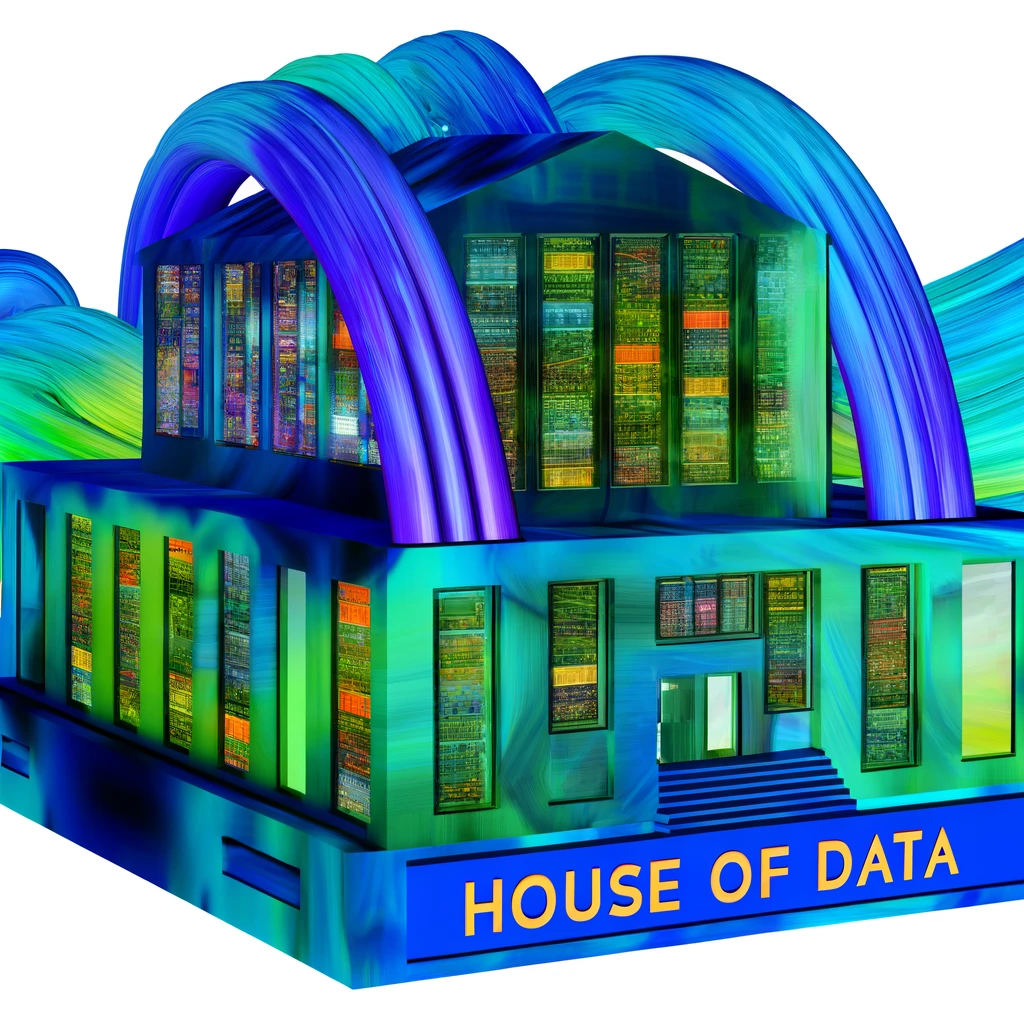
\includegraphics{./houseOfData.webp} \newpage \tableofcontents \newpage

Data to projects are provided from many sources, the most important
being Statistics Denmark (DST) and the Health data organisation
(Sundhedsdatastyrelsen, SDS). Data from these sources are by DST
conceived as ``base data'' (Grunddata) and are systematically placed in
a folder named \textbf{Grunddata}.

All other data will appear in a folder named \textbf{Eksterne data}.
This folder may be further organised depending on the project.

The current listing of dataset is very general and the project you are
working on may contain fewer datasets or additional datasets.

This document provides an overview of the structure of
\textbf{Grunddata}. An important principle for the structure of data has
been to change as little as possible to the orginal data supplied. The
reason for this is that it allows all users to interrogate DST and SDS
for description of registers and definitions of variables. These
institutions have on their web-pages descriptions of datasets and well
as variable explanations.

Register details from the Danish Health Data Authority
(Sundhedsdatastyrelsen) is found here:
\url{https://sundhedsdatastyrelsen.dk/da/registre-og-services/om-de-nationale-sundhedsregistre}
Register details from the Statistics Denmark is found here:
\url{https://www.dst.dk/extranet/forskningvariabellister/Oversigt\%20over\%20registre.html}

A full list of all external data including variable explanations is
found on DDV (Danmarks Data Vindue).

Data management with the new structure will result in changes of many
programs. To ease this process we have written a SAS and R program to
read data in a structured way. These programs are found in
V:/Alle/skeleton and are also visible on www.heart.dk/github/programming
guidance/skeleton.

One very important change for many users is that we provide multiple
files for each register according to the DST habit of having one file
per year. This change is made to ease data organisation as many users
only need to interrogate data from selected years. It further can help
to increase speed of data processing by parallising calculations - the
document \textbf{Parallel processing with SAS and R} describes this.
Also, the programs for SAS/R enabling data management are available in
the folder V:/data/alle/skeleton

The following headlines correspond to the subfolders in
\textbf{Grunddata} on projects.

\hypertarget{cancer}{%
\section{Cancer}\label{cancer}}

This includes the cancer registry from SDS (t\_tumor)

\hypertarget{death}{%
\section{Death}\label{death}}

\textbf{T\_dodsaarsag\_1} is the national cause of death register until
2001 when new death certificates were introduced

\textbf{T\_dodsaarsag\_2} is the new cause of death register. Note that
attempts have been made to provide simple translations of new to olds
cause of death definition, but this should be discouraged. It is
important to note the update of causes of death is very much delayed.

Simple registration of death is in the \textbf{dod} table. This table
combines information from DST (dod) and SDS (t\_person) and is updated
as much as other data in the project. This dataset only cosntained date
of death for deceased and is not described elsewhere.

\hypertarget{krim}{%
\section{Krim}\label{krim}}

This folder contains information on criminal records and and related
subjects. Only available in selected folders.

\hypertarget{laboratory}{%
\section{Laboratory}\label{laboratory}}

This folder first of all holds \textbf{lab\_forsker}. NPU codes
corresponding to tests are found in V:/data/alle/blodprøver.
Additionally there is a dataset \textbf{lab\_labidcodes} which contains
information on the laboratory where the tests were conducted. This may
be useful for selected assays, but carries the caveat that information
on laboratory may not be exported.

Historically we have collected laboratory results from willing sources
and these are placed in separate subdirectories corresponding to the old
municipal of Copenhagen (Kbh amt), Copenhagen general practitioners
laboratory (KPLL), North Region of Denmark and Roskilde. The advantage
of these datasets is that they reach further back in time than
lab\_forsker.

When relevant the \textbf{pato} register of microscope examinations is
also supplied in this directory.

\hypertarget{lpr}{%
\section{LPR}\label{lpr}}

LPR1 uses ICD8-codes and was 1994 replaced with LPR2 and ICD\_10 codes.
This continued until about march 2019 where LPR3 started. LPR3 is
structured very differently from LPR1/2. It has therefore been decided
to maintain the partially digested LPR1/2 data in the following
deliveries: \textbf{diag\_indl} contains all diagnoses and selected
administrative data. \textbf{opr} includes all procedure codes and all
examination codes (sksube) - again with added administrative data.

Some projects will also include \textbf{opr\_old} which are ICD8
procedures prior to approximately 1994. Other projects also have the
file \textbf{lpr\_bes} which are outpatient contacts from lpr2.

Psychiatric admissions were provided in independent tables. Note than
occasionally psychiatric diagnoses appear in the somatic data, but not
consistently.

LPR3 datasets are supplied without changes for the populations relevant
for the project. 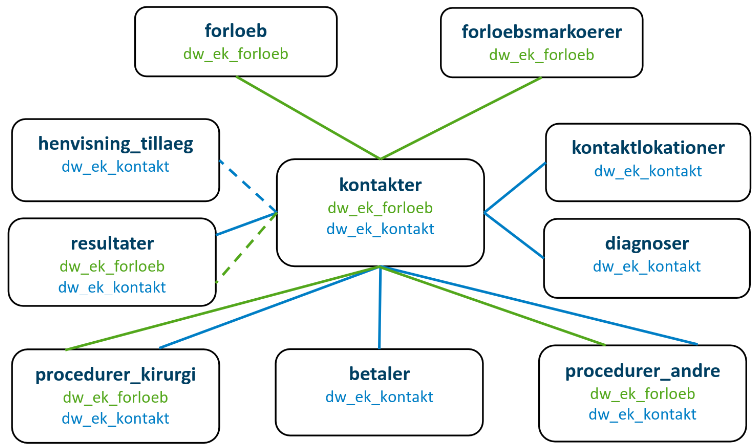
\includegraphics{./lpr3.png} LPR3 contains the datasets
provided in the figure. Additionally the key variables to connect data
are shown. For a short introduction to LPR3 please see:
\url{https://github.com/ctpteam/DST/blob/master/Various\%20Statistics\%20Denmark\%20(DST)\%20manuals/Vejledning\%20til\%20LPR3_F.pdf}

For a thorough introduction to LPR3 see:
\url{https://github.com/ctpteam/DST/blob/master/Various\%20Statistics\%20Denmark\%20(DST)\%20manuals/LPR_Indberetningsvejledning_lang.pdf}

\hypertarget{medication}{%
\section{Medication}\label{medication}}

This directory includes all \textbf{lmdb} files available. Additional
data regarding compounds can be found in
\textbf{laegelmiddeloplysninger}, which in various updated versions are
available on **V:\data\alle\LMDBdata**

\hypertarget{mfr}{%
\section{Mfr}\label{mfr}}

\textbf{mfr} is the national birth register and this dataset has data
from 1997-2019.

We have older data also \textbf{mfr\_lfoed} - born alive prior to 1997
\textbf{mfr\_dfoed} - stillborn prior to 1997 \textbf{nydfoed\_2010} and
\textbf{nylfoed\_2010} are also delivered and may not provide new data.

With the introduction of LPR3 all births from 2019 are found in the
LPR3-table \textbf{nyfoedte}.

\hypertarget{nursinghome}{%
\section{Nursinghome}\label{nursinghome}}

The dataset \textbf{plhjem} is the data we have from nursinghomes
generated by DST by request from us and using the number of old people
at an address to qualify an address to be examined as to whether is was
a nursinghome.

From 2016 the more official data \textbf{aepi} has nursing home data.

The registers \textbf{aefv}, \textbf{aelh}, \textbf{aeph} and
\textbf{aetr} are various types of personal assistance

\hypertarget{population}{%
\section{Population}\label{population}}

The main population register is the \textbf{bef} tables for each year
since 1985 and from 2008 each quater of a year. This is the main
official register to define danish residents at any time.

Prior to 1985 the \textbf{fain} tables provide some of the data found in
\textbf{bef}.

In addition the dataset \textbf{sexBirth} provides date of birth and sex
(0=female,1=male) available from the cpr-register (t\_person). This
particular dataset is not described further elsewhere.

Projects may or may not directly have the \textbf{t\_person} register.
Not that this register also includes legal parents and ``C\_STATUS''
which is 90 for death and also includes information on migration and
people disappeared.

Country of origin is found in the \textbf{iepe} dataset and all
immigrations into and away from Denmark are found in the \textbf{vnds}
table.

\hypertarget{social}{%
\section{Social}\label{social}}

The tables \textbf{indXXXX} hvor Xs represent years include income and
fortune of invididuals. This table also includes individual income
adjusted for family composition. The table does not adjust for
inflation.

The tables \textbf{uddaXXXX} has maximal education for all individuals.
There are SAS formats to translate to understandable values and also a
R-function in heaven to do this.

The table \textbf{uddfXXXX} contains also maximal education. Only the
last year is necessdary to include as it is uptated with new data
annually. It appears to include maximal education for more people than
udda-files, perhaps because imported educations are also registered
here.

The table \textbf{dreamXXXXXX} is an updated version of dream that for
each week has codes indicating public support and for each month
indication of association to particular working areas.

Some projects include \textbf{kotre} and \textbf{koto} which are student
registers. Further educational register may be available in selected
projects.

\hypertarget{sss}{%
\section{SSS}\label{sss}}

\textbf{SYSI} and \textbf{SSSY} are data from practitioners to many
types representing different time periods.

\hypertarget{other-data}{%
\section{Other data}\label{other-data}}

For all projects there is a folder named \textbf{External Data}. The
data in this folder can be found in the description files for the
project - named variables and datasets. Further explanations can be
found in the approvals from DST and SDS or on DDV.

\hypertarget{vdataalle}{%
\section{V:/data/Alle}\label{vdataalle}}

On the V-path subfolder ``alle'' is a number of moderately organised
folders for a variety of anonymous and useful data. Not in particular
details of medication in LMDBdata, text versions of diagnoses in ICD8
and ICD10

Note also here the ``skeleton'' folder that includes sample programs to
import data from the structure required by Statistics Denmark

\hypertarget{dst-formats}{%
\section{DST formats}\label{dst-formats}}

On the desktop of Statistics Denmark there is a STAR called formats.
This provides access to multiple format that can be helpful for
classifying complex codes. For example the four digit final education
can with these data be transformed to ISCED classes.

\end{document}
